\section{Applications of Bandit Problems}
\label{sec:application}
The development of Bandit Problems is rapid, mainly due to its applications and prospects are very impressive.

Early in 1933, Dr. Thompson encountered a difficulty: to treat a same disease, there may be two or even more solutions, but their effectiveness are unknown. Actually, it is also the problem that Bandit problems need to solve, find the best choice on facing some  unknown probability distributions. At that time, Thompson proposed the ``Thompson Sampling''(details in Chapter~\ref{chap:MAB}), a prototype of Bandit problem.
\begin{figure}[!h]
\centering{
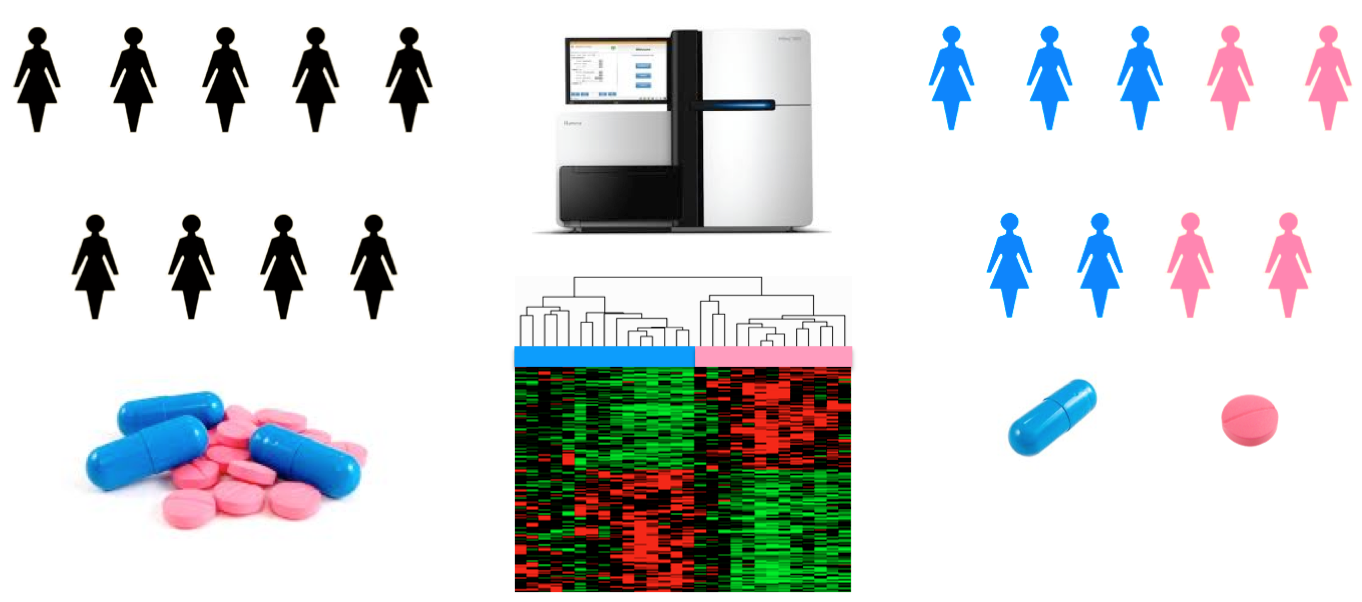
\includegraphics[width=0.6\linewidth]{chapters/chapter01/fig01/clinicaltrials.png}}
\caption{Clinical Trials}
\end{figure}

Nowadays, with the rising development of Internet, the Bandit problems become extremely popular. Such as personalized search, Internet advertising etc. For these applications, Operators will give each user a certain number of recommendations. sometimes, there are some user-friendly, but sometimes not. For traditional way, the supervised learning should get full feedback from users, if there is no interested recommendation. But most users do not like give this full feedback. In this case, Bandit feedback is proposed.(Details will be shown in Chap~\ref{chap:MAB})
\begin{figure}[!h]
%\label{fig:websearch}
\centering{
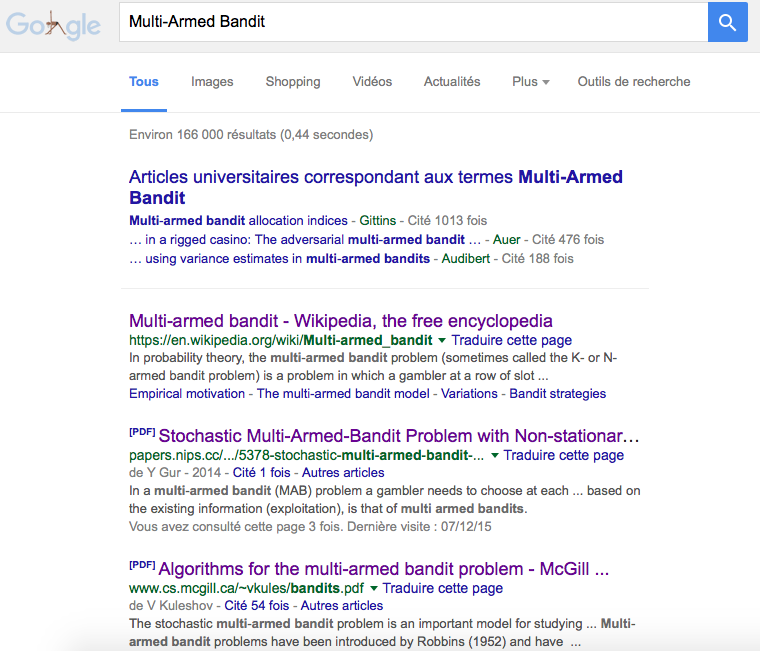
\includegraphics[width=0.6\linewidth]{chapters/chapter01/fig01/websearch.png}
\caption{Web Search}}
\end{figure}

Otherwise, Google proposed an analytic service based on the method of Multi-Armed Bandit(Chapter~\ref{chap:MAB}). It is an analytic system to compare and manage some online experiments. For each experimentation, maybe there are a variety of alternative solutions. In past, it is usually used A/B test to solve, but A/B test cost much and waste time. So google takes Bayes Theorem combining Multi-Armed Bandit, it could reduce much time and get higher accuracy than ever.
\begin{figure}[!h]
\centering{

\includegraphics[width=0.6\linewidth]{chapters/chapter01/fig01/googleanalytic.png}
}
\caption{Google Analytic}
\end{figure}

Except Internet, Bandit problems also have very broad prospects in other domains. Such as in World War II, many countries had tried to solve multi-objective multi-tasking attack, this one could be considered as Multi-Objective Multi-Armed Bandit problem (shown in Chapter~\ref{chap:momab}). Otherwise, queueing and scheduling(\cite{veatch1996scheduling,ehsan2004optimality}), stock in non-stationary(\cite{garivier2008upper}) etc, all of them will be the direction to be committed to develop for Bandit problems.